%----------------------------------------------------------------------------------------
%	ANALISI ARCHITETTURALE
%----------------------------------------------------------------------------------------

\section{Analisi architetturale}
\label{sec:analisi_architetturale}

In questo capitolo verranno presentate le decisioni architetturali inerenti la struttura e l'organizzazione del software di simulazione. L'analisi comincia con una visione generale della gerarchia di eventi, per poi suddividersi nelle scelte che riguardano la parte di concorrenza e le scelte che riguardano la parte di distribuzione.

\subsection{Gli eventi}
\label{sec:analisi_eventi}

Gli eventi sono l'elemento costituente di una partita. Essi possono essere generati dalle diverse entita' e possono essere raggruppati in diverse categorie. Inoltre, alcuni di questi eventi sono interessano la sola parte concorrente, mentre altri eventi possono viaggiare dalla parte concorrente a quella distribuita e viceversa.

\begin{figure}
	\centering
	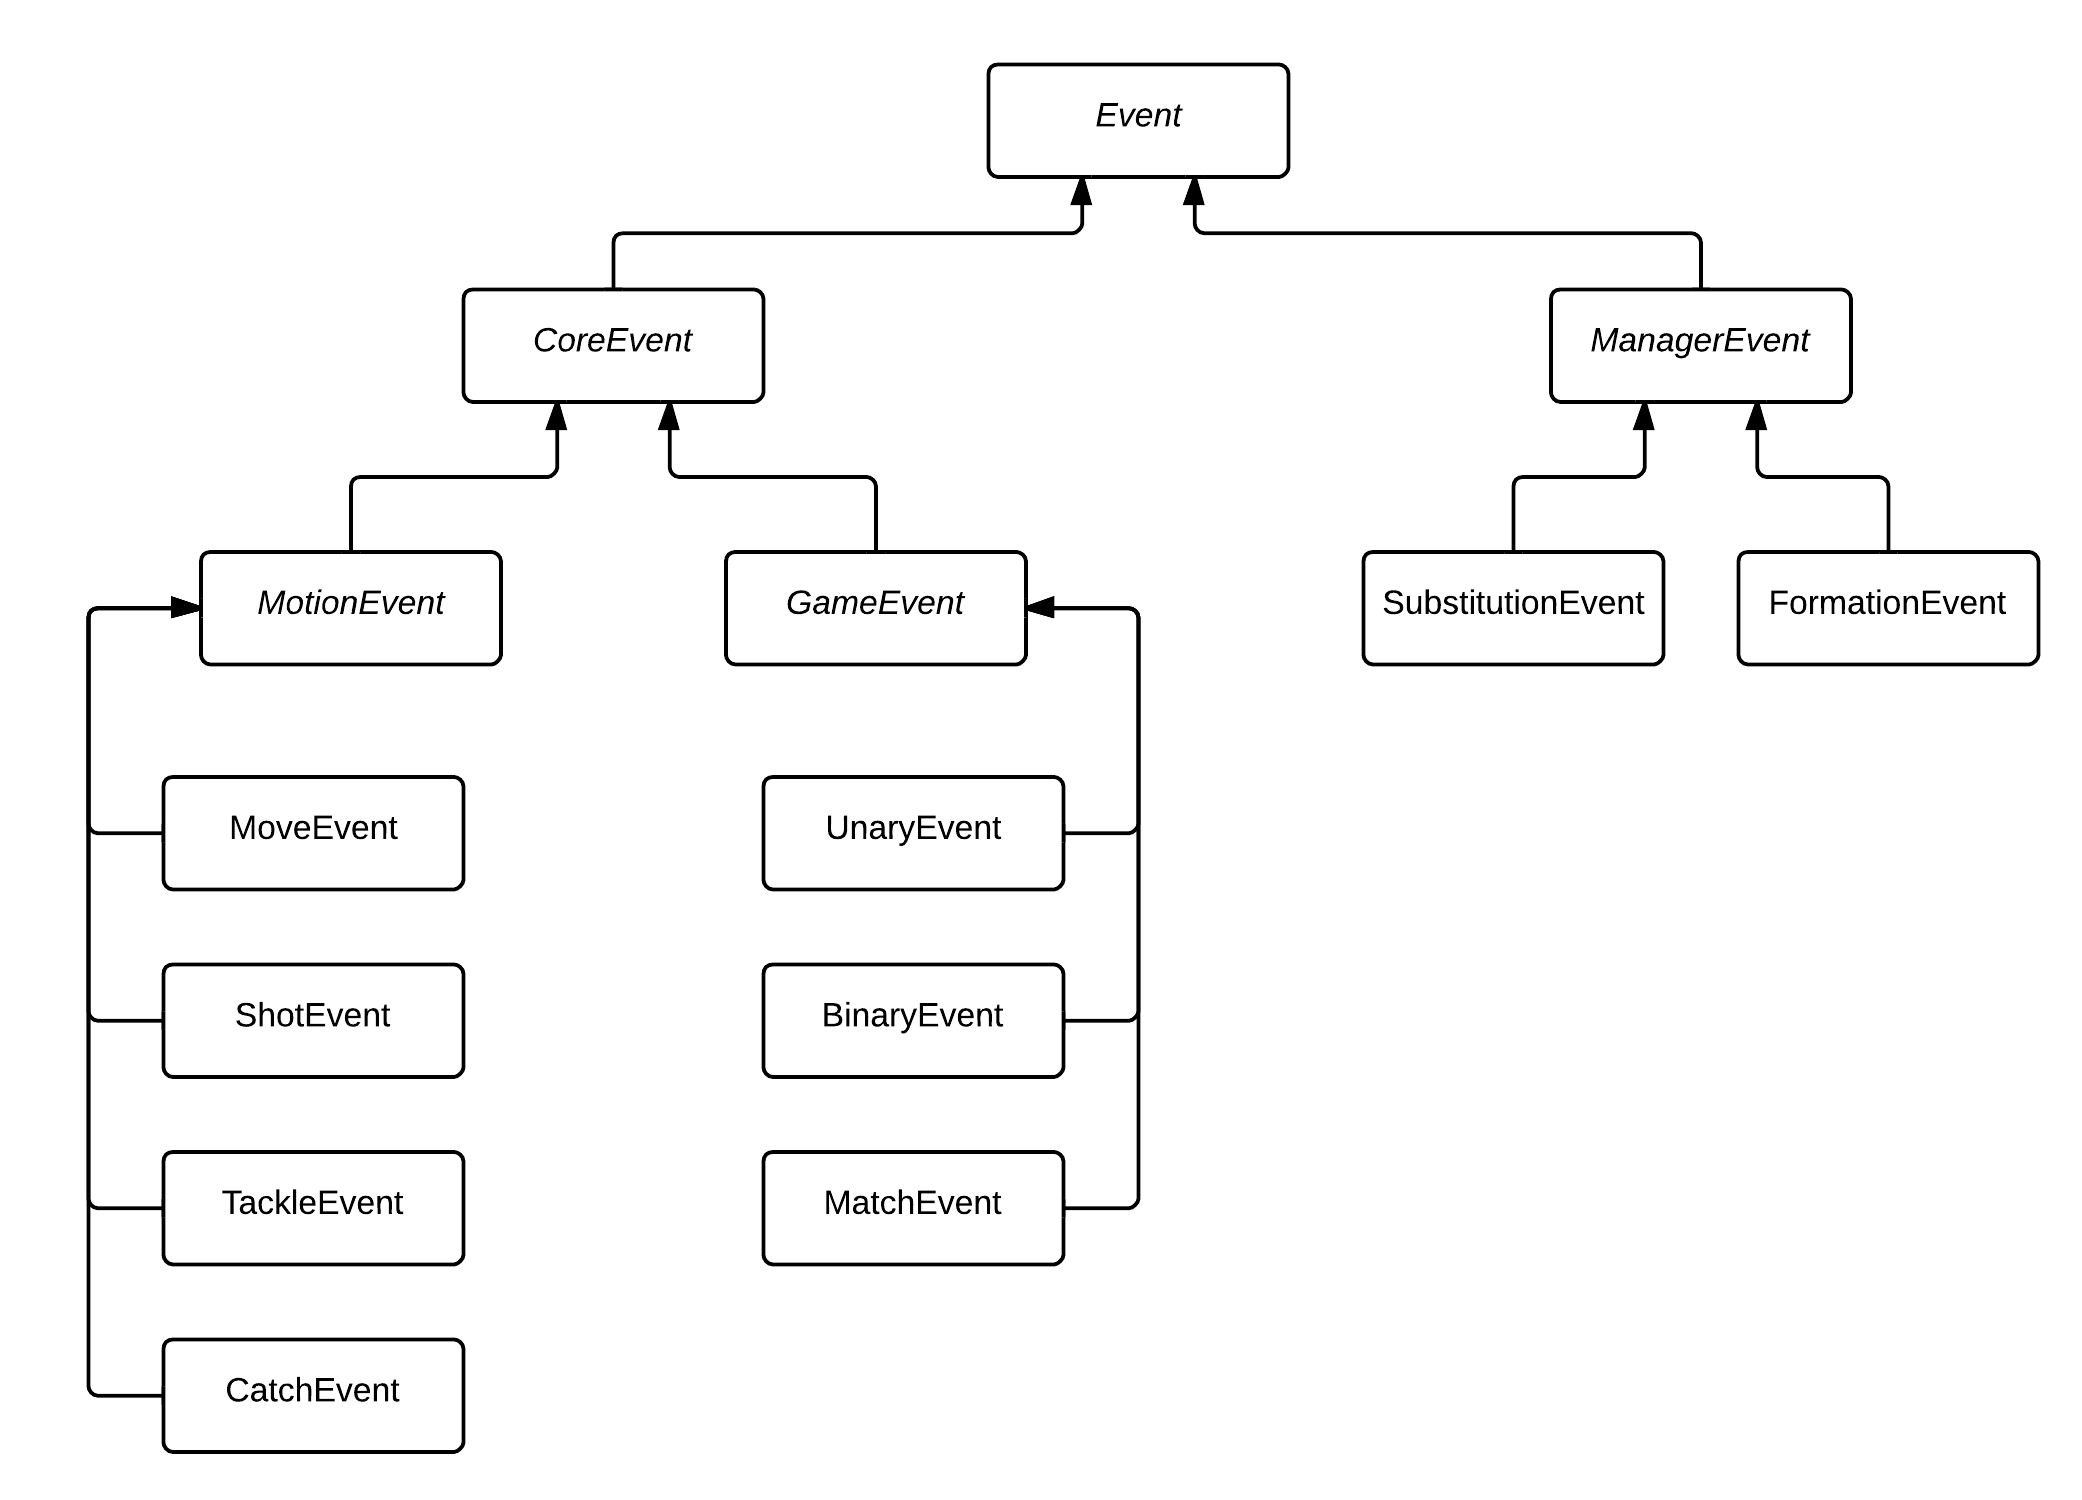
\includegraphics[scale=.5]{images/event_hierarchy.png}
	\caption{La gerarchia degli eventi che costituiscono una partita.}
	\label{fig:event_hierarchy}
\end{figure}

La struttura globale degli eventi e' schematizzata in Figura~\ref{fig:event_hierarchy}. Data la sua complessita' ed estensione, verranno ora trattati singolarmente i diversi tipi di eventi al fine di spiegarne il loro significato e il contesto in cui vengono utilizzati.

\paragraph{Event} \textit{Event} rappresenta l'evento generico ed e' alla base della gerarchia. Da esso si diramano due macro-categorie di eventi: i \textit{CoreEvent} e i \textit{ManagerEvent}. Esso sono rispettivamente gli eventi che vengono generati nella parte concorrente (il cosiddetto ``Core'') e gli eventi che vengono generati nella parte distribuita (fondamentalmente, dagli allenatori). \textit{Event} puo' essere considerata come un'entita' astratta, che non viene concretizzata se non da uno dei suoi derivati.

\paragraph{CoreEvent} Gli eventi di tipo \textit{CoreEvent} sono un insieme di eventi che vengono generati dalla parte concorrente del sistema, ovvero il Core. La loro generazione tuttavia non vincola il loro utilizzo nella sola parte concorrente: essi vengono infatti inviati alla parte distribuita per notificare gli allenatori (e l'interfaccia grafica del campo) sullo svolgersi della partita. Vi sono due tipologie di \textit{CoreEvent}: i \textit{MotionEvent}, che rappresentano le possibili azioni dei giocatori, e i \textit{GameEvent}, che invece rappresentano tutti quelli eventi che influiscono sullo stato di gioco. Anche in questo caso, i \textit{CoreEvent} sono astratti e trovano una concretizzazione nei loro discendenti.

\paragraph{MotionEvent} Tutte le azioni che un giocatore puo' compiere sono definite dai \textit{MotionEvent}. Sono stati definiti quattro tipi di \textit{MotionEvent}, elencati di seguito.

\begin{itemize}
	\item \textit{MoveEvent} - Descrivono i movimenti di un giocatore, dal punto in cui si trova al punto in cui si vuole spostare. Questi eventi vengono altresi' usati per descrivere gli spostamenti della palla.
	\item \textit{ShotEvent} - Rappresentano il tiro/passaggio effettuato da un giocatore, e sono caratterizzati da alcune informazioni quali la posizione del giocatore e la potenza impressa alla palla.
	\item \textit{TackleEvent} - Corrisponde al tentativo di contrasto verso un altro giocatore.
	\item \textit{CatchEvent} - Questo evento descrive il gesto di prendere possesso di una palla, sia essa inerte sul campo (non in possesso) oppure come intercettazione di una palla in movimento.
\end{itemize}

Ciascuno di questi eventi viene sottoposto all'attenzione dell'arbitro, che ne valida la correttezza nel rispetto delle regole del gioco. Inoltre, come gia' anticipato, questi eventi vengono anche inviati alla parte distribuita, cosi' da poter aggiornare la visualizzazione della partita e per permettere agli allenatori di prendere decisioni tattiche.

\paragraph{GameEvent} Gli eventi che regolano lo svolgimento del gioco rientrano nella categoria di \textit{GameEvent}. \\

[TODO] finire la descrizione degli eventi

\subsection{Concorrenza}
\label{sec:analisi_concorrenza}

Una prima panoramica propone la soluzione scelta per garantire l'assenza di deadlock e starvation in fase di design, successivamente viene fatta luce su casi particolari che il modello finora descritto non gestisce così com'è, ma è stato necessario potenziarlo con meccanismi e componenti dedicate.\\

Il software è stato sviluppato con l'utilizzo del linguaggio Ada, il quale ha un modello di concorrenza che ci permette di utilizzare una semantica molto ricca, in particolare mette a disposizione una serie di canali per le richieste che in fase di lettura permettono accessi potenzialmente paralleli, mentre in scrittura vi sono due distinti canali che garantiscono mutua esclusione e in alcuni casi accodamento con condizionale. In particolare quest'ultimo costrutto è molto utile quando si vuole soddisfare una richiesta solamente al verificarsi di alcune condizioni, per esempio una risorsa che si libera o il cambiamento dello stato di gioco.

\subsubsection{Deadlock, starvation e correttezza}
\label{sec:analisi_concorrenza_deadlock}

In un sistema concorrente è necessario tenere conto di problematiche come la starvatin ed il deadlock quando si è in presenza di entità che condividono risorse. Nel caso di questo progetto i giocatori devono avere accesso ad uno stato condiviso che gli permetta di prendere decisioni con le quali andare ad aggiornare lo stato stesso.\\

L'analisi ha evidenziato la necessità di avere un unico luogo in cui mantenere lo stato, ed in fase di modellazione tale problematica è stata risolta ponendo un'unica entità che garantisce mutua esclusione a controlloro dei dati condivisi.\\

Questa decisione rente più semplice garantire l'assenza di deadlock e starvation. Nel secondo caso ogni job ha garanzia di accedere alla risorsa in un tempo finito in quanto le richieste vengono processate con ordinamento FIFO basato sull'orario di arrivo. Per quanto riguarda il deadlock solamente una delle quattro condizioni perchè si verifichi tale condizione. I giocatori eseguono la sequenza di operazioni che caratterizza un turno dividendole tra “online” ed “offline”, cioè solamente le fasi di lettura e di scrittura necessitano dell'utilizzo della risorsa, mentre la parte di intelligenza artificiale viene effettuata in modo autonomo sui dati recuperati. Inoltre solamente la parte di scrittura richiede mutua esclusione. I prerilascio non è inibito ed il suo comportamento non è controllato dal software ma dal sistema operativo operativo sottostante, un job prerilasciato che esta eseguendo la sezione critica di una richiesta in mutua esclusione al suo risveglio deterrà ancora il privilegio sulla risorsa, mentre gli altri job che la richiedono saranno in attesa sul canale esposto. Caso più particolare invece per quanto riguarda attesa circolare ed accumulo di risorse, in questo caso entra in gioco un meccanismo di riaccodamento e rivalutazione delle richieste che viene discusso in seguito, il concetto alla base è che una richiesta che non viene soddisfatta a causa di una risorsa occupata può fallire o riaccodata per essere ritentata di in un secondo momento, in questo caso dopo un numero di tentativi l'operazione viene rivalutata e modificata in una simile che soddisfi comunque le esigenze del giocatore.

\subsubsection{Palla}
\label{sec:analisi_concorrenza_palla}

La palla consiste in una risorsa protetta che ne detiene la posizione e ne permette l'accesso in mutua esclusione. Supponiamo di tenere tale risorsa all'interno del controllore, cioè permettendo solo ad esso di accederla, in questo caso sia giocatori che agente di movimento devono concorrere per andare a modificare lo stato, quindi anche la posizione della palla, ponendo quindi il moto del pallone allo stesso livello delle decisioni e spostamenti dei giocatori. In queste circostanze verrebbe meno un fattore di realismo secondo cui il pallone è slegato dalla velocità di gioco dei giocatori in campo, esso deve essere libero di muoversi a velocità molto più alte ed anche a gioco fermo, fino a che non sarà l'arbitro a riposizionarla (per fare un esempio) nel punto del fallo o della rimessa. Inoltre accodando la richiesta di movimento della palla durante un tiro insieme alle richieste dei giocatori rende le operazioni prettamente sequenziali, mentre vi sono aspetti in cui il parallelismo aggiunge un livello di indeterminismo al simultatore che lo fa avvicinare al gioco reale.\\

Un esempio è il tentativo di un giocatore di prendere la pallla in movimento, è ragionevole pensare la sua azione possa fallire perchè magari il tiro è troppo forte, ponendo palla e stato in due luoghi differenti è possibile che mentre il giocatore prova a prendere il pallone che secondo lui si trova in una certa posizione quest'ultima si stata spostata più avanti, rendendo vano il suo tentativo.\\

Sulla base delle considerazioni fatte, all'interno dell'architettura e' stato deciso di tenere le informazioni riguardanti la palla slegate rispetto al controllore. Permettendo così sia ad un giocatore che all'agente di movimento di contenderla potenzialmente in modo parallelo, demandando alla risorsa che identifica la palla gestirne gli accessi in mutua conclusione e sotto determinate circostanze.\\

La struttura della palla e' stata quindi studiata in modo tale da permettere ad un entita' alla volta di poterla controllare, quindi o uno dei giocatori o l'agente di movimento, quest'ultimo si attiverà quando risvegliato da un giocatore e fermato quando un altro conquista il pallone o se il moto che gli era stato impresso si è esaurito. Quest'utlimo aspetto sfrutta la potenza dei canali che permettono accodamento con condizione per attivare e disattivare il task.

\subsubsection{Giocatori}
\label{sec:analisi_concorrenza_giocatori}

I giocatori dopo una fase di inizializzazione eseguono ad ogni turno un'operazione che va a modificare lo stato di gioco oltre che al proprio. Se ogni giocatore avesse la propria parte di stato, renderebbe complicato la condivisione di esso con le altre entità in gioco, inoltre la necessità di un unico stato centrale rende tali informazioni ridondanti oltre che difficilmente consistenti durante l'esecuzione della simulazione.\\

\textbf{Task stateless}\\

Utilizzando un approccio in cui i giocatori sono stateless si permette una migliore gestione dei dati condivisi mantenendoli solamente in un unico luogo all'interno del sistema, ad ognuno dei 22 task in campo viene assegnato un id con il quale ad ogni turno ottiene le informazioni di cui necessita. Tale identificatore viene ottenuto in fase di inizializzazione e puo' cambiare in caso di sostituzione tra un giocatore in campo ed uno in panchina, in questo modo non vi e' la necessita' di creare o risvegliare un secondo task.\\

\textbf{Area di azione}\\

Ogni giocatore e' caratterizzato da delle statistiche impostate in fase di inizializzazione che lo differenziano dagli altri, ed ha come scopo quello di rendere lo svolgimento del gioco piu' realistico. Tali statistiche comprendono potenza, velocita', contrasto, difesa, attacco, precisione e bravura in porta. Abbianate allo stato di gioco dello stesso giocatore, rendono possibile effettuare alcune assunzioni che influiscono nello svolgimento del resto del turno. \\

Se un giocatore possiede la palla e tra le proprie statistiche ha un'alta precisione e potenza, esso potra' effettuare un lancio lungo, in caso contrario potra' optare un passaggio corto ad un compagno vicino. Viene definita in questo modo un'area di interesse del giocatore, entro la quale esso potra' agire a prescindere dall'azione che scegliera' di fare. Un giocatore che chiede al controllore lo stato di gioco della partita non necessita di avere una visione globale dell'intero campo, bensi' solamente di una sua sotto parte, definita dalla sua posizione ed un raggio determinato in base alle caratteristiche del giocatore ed alle informazioni preliminari che ha ottenuto riguardo allo stato globale.\\

\textbf{Il turno}\\

La parte iniziale di ogni turno del giocatore risulta' cosi' suddivisa:

\begin{enumerate}
	\item richiesta al controllore del proprio stato di gioco
	\item dove si trova la palla
	\item richiedere al controllore lo stato della propria area di interesse.
\end{enumerate}

Queste operazioni, in quanto letture, avvengono effettuate potenzialmente in modo parallelo rispetto agli altri task.\\

La seconda fase consiste nella parte di intelligenza artificiale nella quale viene decisa la . Una volta decisa la mossa da effettuare, viene creato il relativo evento a cui abbina un certo livello di priorita', cioe' quanto e' importante per il giocatore l'azione appena decisa. L'azione composta da evento e priorita' vengono sottoposte al controllore tramite una chiamata in mutua esclusione con accodamento. Tale canale viene sfruttato dal sistema per fermare il gioco e farlo riprendere, per esempio quando l'utente mette in pausa il gioco.\\

Antecedente al ciclo di turni che caratterizzano la normale esecuzione di un giocatore e' presente una fase di inizializzazione nella quale il giocatore attende che tutti i giocatori siano attivi, recupera il proprio id ed attende l'inizio della partita.\\

Ci sono altri casi in cui vi e' la necessita' di fermare per poi far ripartire i giocatori, in questi casi viene fatto uso di una risorsa protetta che mette a disposizione dei canali per accodare i giocatori per poi sboccarli al verificarsi di determinate condizioni.\\

\textbf{Entrata in campo}\\

L'entrata in campo come l'uscita e' un altro degli aspetti critici della concorrenza del progetto. I giocatori sono creati con posizione di partenza sulla panchina della propria squadra, che consistono in una serie di celle esterne al campo, ed all'avvio della partita si spostano verso la propria posizione. In una partita reale i giocatori entrano ed escono dal terreno di gioco dal centro del lato lungo, per avere questo comportamento e' stata inserita una cella di campo esattamente adiacente al punto desiderata attraverso la quale i giocatori passano dalla panchina al campo e viceversa.\\

\textbf{Sostituzione}\\

La cella utilizzata nel meccanismo di entrata ed uscita dal campo viene sfruttata per effettuare le sostituzioni, un giocatore che deve essere sostituito dopo essersi accorto tramite lettura dello statao esce fino a raggiungere tale cella, in essa il suo id viene cambiato con quello del nuovo giocatore. Dato che i giocatori non hanno stato, se non l'id che li identifica e con il quale recuperano ad ogni turno le proprie informazioni dal cotroller, modificando il suo valore e' equivalente ad averlo sostituito. In questo modo vengono creati solamente 22 giocatori in ogni partita, riutilizzandoli per simulare quelli in panchina.\\

\subsubsection{Stato, controllor ed arbitro onniscente}
\label{sec:analisi_concorrenza_controller_arbitro}

Lo stato consiste in una serie di dati che descrivono ogni giocatore in campo, quindi un identificativo, il numero di maglia, la posizione attuale e quella di riferimento in campo (cioe' la posizione dettata dalla formazione), oltre ad informazioni generali sullo stato nel suo complesso. Lo scopo delle azioni da parte dei giocatori e' quella di andare a modificare la propria posizione all'interno del campo ed effettuare altre operazioni ai fini del gioco.\\

Il controllore gestisce gioco tramite la sua componente di arbitro influenzando l'andamento  del gioco, quando necessario blocca la ricezione di richieste scrittura di eventi.\\

\textbf{Arbitro}\\

Ogni richiesta viene presa in cosiderazione dalla componente che rappresenta l'arbitro, il quale valuta la correttezza o meno dell'azione. In caso di fallo l'arbitro ferma il gioco dal punto di vista logico e sancisce la squadra per il prossimo possesso palla. A questo punto prima che il gioco possa riprendere l'arbitro attende che le squadre si riposizionino correttamente per garantire le giuste distanze dal punto di battuta, poi il gioco riprende al momento di battuta da parte del giocatore designato.\\

\textbf{Processare eventi}\\

Nel sistema esistono diversi tipi di eventi e di azioni che un giocatore puo' efffettuare, dal punto di vista del controllore vengono gestite in modo differente: una volta accettata la richiesta ne determina il tipo e cerca di soddisfare il giocatore permettendogli di aggiornare lo stato con l'azione richiesta. Il fatto che il giocatore divida il suo turno in fasi, fa in modo che i presupposti secondi cui ha scelto una determinata mossa al momento non vi siano piu'.\\

Per esempio, un giocatore tenta di prendere la palla che e' in una certe posizione, ma tra quando se ne e' accorto e quando tenta effettivamente di prenderne il possesso, la palla si e' spostata. Questo, come anche in altri casi in cui ha senso applicare questo tipo di comportamento, e' dettata dal tentativo di creare una simulazione realistica, se un giocatore non e' abbastanza veloce o si accorge tardi di una certa circostanza e' giusto che veda la propria azione fallire.\\

Se l'operazione fallisce, cioe' non puo' essere applicata allo stato, il controllore si comporta in modo differente in base al tipo di operazione richiesta:

\begin{itemize}
	\item operazioni come il passaggio, il tiro, il tentativo di prendere la palla ad un avversario o mentre non e' controllata da nessun giocatore se non vanno a buon fine falliscono, il giocatore al turno successivo si accorge che lo stato non e' stato modificato come aveva richiesto
	\item le operazioni di movimento possono fallire, la cella di destinazione potrebbe essere stata occupata, sotto certe condizioni tale mossa puo' essere ritentata in seguito
\end{itemize}

L'utilita' che un giocatore assegna alla propria azione determina il comportamento nel secondo caso, la richiesta quando accettata dal controllore ha una certa utilita', se non va a buon fine questo valore viene decrementato e la mossa messa in attesa di una nuova occasione di esecuzione. Ad ogni tentativo il valore decresce fino a diventare minore di una certa soglia fissata priori, sotto la quale l'azione richiesta viene rivalutata dal controllore. Questo consiste nel soddisfare la richiesta con un'operazione il piu' simile possibile a quella decisa dal giocatore.\\

Tale meccanismo ha come scopo quello di riflettere cio' che succede nelle dinamiche di una partita reale, se un giocatore vuole raggiungere una certa posizione, ma nel percorso che vuole fare si trova un altro giocatore, per un po' temporeggiera' nell'attesa di un suo spostamento, poi cambiera' leggermente la propria corsa per evitare l'ostacolo.\\

Nella descrizione del meccanismo manca un particolare, cioe' quando un azione fallita viene ritentata. Un azione di movimento per poter essere di nuovo sottoposta al controllore necessita che il giocatore che la impedisce si sia spostato, ma tale approccio potrebbe risultare troppo oneroso dal punto di vista implementativo e poi a tempo di esecuzione. La soluzione scelta consiste di permettere la rivalutazione delle mosse fallite ogni qual volta che un giocatore lascia la propria posizione, anche se non e' detto che sia quella desiderata da un giocatore. Per rendere questo meccanismo piu' efficiente e' stato suddiviso il campo di gioco in 6 settori, quindi ogni richiesta che non e' andata a buon fine e deve essere ritentata viene accodata sulla zona in cui si trova il giocatore, in attesa che un altro giocatore di quella zona effettui un movimento. In questo modo non vengono rivalutate tutte le richieste accodate all'interno del controllore, ma solamente quelle che potenzialmente ora sono applicabili.\\

Questi meccanismi nel loro insieme permettono di non avere dead-lock, cioe' che un giocatore non resto bloccato in attesa di una risorsa che al momento della richiesta non era disponibile.

\subsubsection{La velocita'}
\label{sec:analisi_concorrenza_velocita}

Nello svolgimento del gioco descritto finora le caratteristiche entrano in gioco quando i giocatori entrano in contatto tra di loro, per esempio contrasto ed attacco quando il difensore tenta di rubare il pallone all'attaccante, la precisione e la potenza quando due compagni vogliono passarsi il pallone o tirare in porta, la parata per evitare che la propria squadra prenda gol, e cosi' via. In tutti questi casi e' il controllore che quando esamina la richiesta di una determinata azione considera i valori dei vari giocatori, decidendo quindi chi vincera' il contrasto, quanto preciso sara' il passaggio, quanto forte applicare al tiro.\\

Per quanto riguarda la velocita' e' necessario un approccio differente, essa si esprime come la quatita' di mosse che e' in grado di fare in un lasso di tempo, quindi quante richieste puo' sottoporre al controllore in questo frangete. Per semplicita' di esposizione tale quantita' di tempo e' identificata dal simbolo $T$, mentre con $t_0$, $t_1$, $t_2$,... indichiamo gli istanti a distanza $T$ durante lo svolgimento del gioco.\\

Ad ogni giocatore e' abbinato un valore tra 1 e 5 per indicare quante mosse sono permesse durante $T$, quindi il giocatore con piu' mosse a disposizione sara' piu' veloce rispetto ad un numero minore. Questo rispecchia quanti turni deve poter eseguire, diventa quindi cruciale come viene calcolato $T$, esso deve permettere ad ogni giocatore di eseguire un numero di volte pari al suo valore che rappresenta la velocita'. Dato un campionamento del tempo di esecuzione pessimo di un turno di un giocatore, che chiameremo C, vogliamo che un giocatore lento esegua $C$ una volta all'interno di $T$, uno un po' piu' veloce due volte, e cosi' via fino a 5. Inoltre vogliamo che all'inizio di ogni $T$, al tempo $t_i$, tutti i giocatori siano pronti per eseguire il proprio turno, questo aggiunge al gioco un ulteriore livello di indeterminismo, in quanto non e' possibile sapere quali saranno i giocatori selezionati per eseguire per primi.\\

Da questo ragionamento si ottiene che $T$ e' pari alla somma di tutti questi tempi, quindi del tempo di tutte le esecuzioni di $C$ da parte di ogni giocatore in campo. In questo modo si garantisce ad ogni giocatore un tempo di esecuzione sufficiente per portare a termine i propri turni, spetta poi ad ognuno di essi distribuirli in modo uniforme nell'arco di $T$, tramite un sistema di delay che scandisce il tempo ripartendolo. Un esempio, poniamo $T$ pari a 40 unita' di tempo ed iniziato al tempo $t_i$, $C$ uguale a 2 e la velocita' pari a 5: il giocatore tra un turno e l'altro tentera' di eseguire il suo turno entro le prime 8, 40 diviso 5, unita' di tempo, per poi attendere fino a $t_i$ + 8 per il prossimo turno. Non e' detto che esso riesca ad eseguire per 2 unita' di tempo nel periodo di 8, dato che i giocatori iniziano ad eseguire tutti insieme, ma di sicuro eseguira' 5 volte il tempo $C$ (2) all'interno dell'iperperiodo $T$ (40).\\

Dato $C$ come stima fatta a priori, in questo meccanismo il controller ha il compito di calcolare $T$ e tenere aggiornato il tempo $t_i$ di riferimento. $T$ e' il pari alla somma di tutti i turni di ogni giocatore, il controllore deve calcolare tale valore ad inizio del gioco, per poi aggiornarlo ogni qual volta ce ne sia il bisogno, per esempio in caso di sostituzione con un giocatore con un altro, questo perche' non e' detto che abbiano la stessa velocita'. Per quanto riguarda $t_i$, in un
a normale esecuzione della partita tale valore viene calcolato partendo da un tempo di riferimento all'avvio del software, al quale viene aggiunto ogni volta $T$, in caso invece di interruzione del gioco da parte dell'utente tale valore di riferimento deve aggiornato con l'istante in cui il gioco puo' riprendere.\\

[TODO esempio di iperperiodo grafico]

\subsection{Distribuzione}
\label{sec:analisi_distribuzione}

Dal momento che la componente \textit{Core} non dispone di una propria interfaccia grafica che possa garantire la fruizione e l'interazione dall'esterno, si pone la necessita' di rendere possibile una comunicazione bidirezionale da e per le componenti distribuite, ovvero \textit{Field} e le due istanze di \textit{Manager}. Di seguito verranno quindi analizzate le soluzioni adottate per questo particolare aspetto del software, la cui rispettiva implementazione verra' successivamente trattata nel Capitolo~\ref{sec:implementazione}.

\subsubsection{Il bridge}
\label{sec:analisi_distribuzione_bridge}

Il modulo che si occupa di consentire alla componente \textit{Core} di accettare comunicazioni dall'esterno, sia in entrata che in uscita, e' chiamato \textit{bridge}. A causa della duplice natura delle comunicazioni possibile, il bridge e' logicamente diviso in due parti: bridge input e bridge output.

\paragraph{Bridge input}\label{sec:analisi_distribuzione_bridge_input} Il bridge input viene utilizzato dalle due componenti distribuite \textit{Field} e \textit{Manager} per comunicare con la componente \textit{Core}, occupandosi quindi di gestire tutte le comunicazioni in ingresso. Per quanto riguarda \textit{Field}, i metodi a sua disposizione permettono di:

\begin{itemize}
	\item Iniziare una nuova partita
	\item Mettere in pausa la partita corrente
	\item Dare il via al secondo tempo, a seguito di un intervallo
	\item Terminare la simulazione (spegnimento globale del software)
\end{itemize}

\noindent Per quanto riguarda invece la componente \textit{Manager}, e' possibile:

\begin{itemize}
	\item Recuperare tutte le informazioni relative ad una squadra
	\item Recuperera tutte le informazioni relative ai giocatori
	\item Cambiare la formazione della squadra
	\item Effettuare una sostituzione tra due giocatori
\end{itemize}

Appare tuttavia evidente che la separazione logica tra le due tipologie di bridge non rispecchia il flusso dei dati trasmessi: infatti, nel caso del bridge input, esso permette alle componenti distribuite sia di richiedere informazioni (e.g. recuperare le statistiche dei giocatori) che di inviare delle informazioni (e.g. cambiare la formazione).\\

\paragraph{Bridge output}\label{sec:analisi_distribuzione_bridge_output} Il bridge output viene invece utilizzato da \textit{Core} per notificare gli avvenimenti della partita, permettendo cosi' a \textit{Field} e \textit{Manager} di disegnare l'interfaccia grafica e di mostrare le relative informazioni. Questo modulo gestisce quindi tutte le comunicazioni in uscita; inoltre, il flusso di dati trasmessi e' solo uscente, a differenza della sua controparte.\\

Alla base del bridge output e' posto un buffer, il cui compito consiste nel raccogliere tutti gli eventi di gioco che vengono generati durante una partita ed inviarli periodicamente alle componenti distribuite. Il contenuto del buffer viene inviato se si verifica una tra tre particolari condizioni. Banalmente, il fatto che il buffer si riempia completamente causa l'invio di tutti gli eventi e un conseguente svuotamento dello stesso. Se invece il buffer non riceve piu' eventi entro un certo periodo di tempo noto a priori, viene inviato il tutto contenuto del buffer (e viene svuotato). Infine, vi sono eventi piu' importanti di altri che devono essere notificati immediatamente (e.g. una fallo): anche in questo caso, il sopraggiungere di uno di questi eventi scaturisce l'invio di tutti gli eventi e lo svuotamento conseguente del buffer.\\

Ad ogni modo, la scelta della dimensione del buffer e' molto importante e determina il throughtput degli eventi e la conseguente ``fluidita\''' della rappresentazione grafica della partita. Tuttavia, un invio piu' frequente di eventi puo' essere causa di una congestione di rete, quindi e' opportuno trovare un buon bilanciamento tra quantita' di eventi inviati e frequenza di invio. A questo proposito, il bridge output applica una sorta di filtraggio degli eventi nel tentativo di unire piu' eventi in uno unico. Questo avviene molto spesso negli eventi di movimento dei giocatori e della palla, che sono in assoluto i piu' frequenti durante una partita. La tecnica che il bridge output adotta e' quella di unificare delle mosse successive di uno stesso giocatore (o della palla) in un unico evento, che ha come punto di partenza quello del primo evento ricevuto e come punto di destinazione quello dell'ultimo evento ricevuto. In questo modo il numero di eventi e' di gran lunga inferiore e garantisce maggior efficienza senza inficiare sulle performance e sul throughtput.

\paragraph{Utilizzo del bridge}\label{sec:analisi_distribuzione_bridge_utilizzo} Il bridge, poiche' risiede all'interno di \textit{Core}, deve essere necessariamente acceduta ed utilizzata da una delle entita' presenti in quella componente. Inoltre, dal momento che le comunicazioni dall'esterno sono asincrone e non predicibili, che l'accesso avvenga serialmente, sia esso in lettura o in scrittura. Per garantire questa caratteristica l'unica entita' che si occupa di interagire con il bridge e' l'arbitro (ai fini della spiegazione lo si consideri come un sotto-modulo del controllore). Per facilitare la comprensione delle interazioni dell'arbitro con il bridge, si consideri la seguente situazione, dove il controllore ha appena eseguito un'azione proveniente da un giocatore e la sottopone all'attenzione dell'arbitro. Quest'ultimo esegue le seguenti operazioni:

\begin{enumerate}
	\item Controlla se l'azione puo' causare una situazione di gioco fermo (che, si ricorda, permette ad una sostituzione e ad un cambio di formazione di avvenire)
	\item Interroga il bridge input e controlla se ci sono richieste da parte della distribuzione; in caso affermativo, le esegue, se le condizioni lo permettono
	\item Valida l'azione del giocatore e aggiunge il rispettivo evento alla coda del buffer di bridge output
	\item Se tale azione ne causa un'altra (e.g., un goal), l'evento di quest'ultima viene aggiunto alla coda del buffer di bridge output
\end{enumerate}

L'ordine in cui queste operazioni vengono eseguite rispecchia l'ordine nel quale vengono processate in una vera partita di calcio. Inoltre, essendo l'accesso al bridge riservato al solo arbitro, vengono evitate potenziali inconsistenze sullo stato della partita.\\

L'unica eccezione a questa regola e' costituita dagli eventi della distribuzione che agiscono sullo stato generale del sistema, ovvero la richiesta di una nuova partita, di mettere in pausa quella corrente oppure di terminare la simulazione ed il sistema. In questo caso e' direttamente il bridge input ad impartire il relativo comando, senza quindi aspettare che sia l'arbitro ad accorgersi della richiesta; tale scelta e' stata dettata dal fatto che questa tipologia di richieste ha la massima priorita' sulle altre, in quanto agisce sul sistema stesso.

\subsubsection{Architettura client-server}
\label{sec:analisi_client_server}

\subsubsection{Architettura publisher-subscriber}
\label{sec:analisi_client_pusblisher_subscriber}